  %%%%%%%%%%%%%%%%%%%%%%%%%%%%%%%%%%%%%%%%%%%%%%%%%%%%%%%%%%%
\documentclass[14pt]{extreport}

% 1. Cores e pacotes gráficos (devem vir PRIMEIRO)
\usepackage[usenames,dvipsnames,svgnames]{xcolor}
\usepackage{graphicx}
\usepackage{epsfig}
\usepackage{pgf,tikz}
\usetikzlibrary{calc,decorations.pathreplacing}
\usepackage{tkz-euclide}

% 2. Linguagem e codificação
\usepackage[utf8]{inputenc}
\usepackage[brazil]{babel}

% 3. PythonTeX
\usepackage{pythontex}

% 4. Matemática e fontes
\usepackage{amsfonts,mathtools,amsthm,amssymb}
\usepackage{stmaryrd}

% 5. Layout, tabelas e formatação
\usepackage{fancyhdr}
\usepackage{makeidx}
\usepackage{enumerate}
\usepackage{wrapfig}
\usepackage{xspace,setspace}
\usepackage[rm]{titlesec}
\usepackage[hmargin=1cm,vmargin=1.5cm]{geometry}
\usepackage{tabu}
\usepackage{multicol}
\usepackage{ccicons}
\usepackage{makecell}
\usepackage[nodayofweek]{datetime}

% 6. Caixas (tcolorbox)
\usepackage[many]{tcolorbox}
\tcbuselibrary{theorems}

% 7. Hyperref (DEVE vir por último entre os pacotes de formatação)
\usepackage{hyperref}
\hypersetup{
    colorlinks = true,
    urlcolor   = cyan,
    linkcolor  = red,
    citecolor  = blue
}

% 8. Licença
\usepackage[
type={CC},
modifier={by-nc},
version={4.0},
lang={brazilian},
]{doclicense}

% Configurações gerais
\renewcommand{\baselinestretch}{1.2}
\allowdisplaybreaks
\makeindex
%\nonstopmode

%----------------- Caixa de Teoremas (tcolorbox) --------------------------
\newtcbtheorem[number within=chapter]{theoremb}{Teorema}%
{
    enhanced,
    drop fuzzy shadow,
    colback=blue!5!white,
    colframe=blue!50!black,
    fonttitle=\bfseries,
    coltitle=white,
    description delimiters parenthesis,
    separator sign none
}{teo}

\newtcbtheorem[use counter from=theoremb]{exeb}{Exemplo}%
{
    enhanced,
    drop fuzzy shadow,
    colback=green!5!white,
    colframe=green!50!black,
    fonttitle=\bfseries,
    coltitle=white,
    description delimiters parenthesis,
    separator sign none
}{exe}

\newtcbtheorem[use counter from=theoremb]{exerb}{Exercício}%
{
    enhanced,
    drop fuzzy shadow,
    colback=red!5!white,
    colframe=red!50!black,
    fonttitle=\bfseries,
    coltitle=white,
    description delimiters parenthesis,
    separator sign none
}{exer}

%----------------- Teoremas Padrão --------------------------
\newtheorem{theorem}{Teorema}[chapter]
\newtheorem{lemma}[theorem]{Lema}
\newtheorem{corollary}[theorem]{Corolário}
\newtheorem{proposition}[theorem]{Proposição}

\theoremstyle{definition}
\newtheorem{definition}[theorem]{Definição}
\newtheorem{example}[theorem]{Exemplo}
\newtheorem{xca}[theorem]{Exercício}

\theoremstyle{remark}
\newtheorem{remark}[theorem]{Observação}

\numberwithin{section}{chapter}
\numberwithin{equation}{chapter}

%----------------- Novos Comandos --------------------------
\newcommand{\R}{\mathbb{R}}
\newcommand{\N}{\mathbb{N}}
\newcommand{\C}{\mathbb{C}}
\newcommand{\dt}[1]{{\color{blue}\textbf{#1}}}
\newcommand{\ep}{\varepsilon}
\newcommand{\nl}[1]{\|#1\|_{\mathcal{L}(X)}}
\newcommand{\dm}{d}
\newcommand{\vt}[1]{\overrightarrow{#1}}

\newcommand{\marcador}[2]{%
    \phantomsection%
    \addcontentsline{toc}{#1}{#2}%
    \noindent {\large \textbf{#2}}\par\vspace{1em}%
}

\newcommand{\n}[1]{\|#1\|}

\DeclareMathOperator{\rank}{\operatorname{rank}}
\DeclareMathOperator{\im}{Im}
\DeclareMathOperator{\id}{I}
\DeclarePairedDelimiterX{\inp}[2]{\langle}{\rangle}{#1, #2}


%----------------- Caixa de Sombra (Substituto do \shadowbox) --------------------------
\newtcbox{\myshadowbox}{
  enhanced,
  sharp corners,
  colback=white,
  colframe=black,
  boxrule=0.5pt,
  shadow={2pt}{-2pt}{0pt}{black}, % Reproduz a sombra clássica do \shadowbox
  boxsep=0pt,
  left=4pt, right=4pt, top=4pt, bottom=4pt,
  nobeforeafter,
  tcbox raise base
}

%----------------- Estilo do Capítulo --------------------------
\font\largefont= pzcmi scaled 3500
\font\numberfont= pzcmi scaled 3000

\titleformat{\chapter}[display]
  {\normalfont\Large}
  {\filright
    \rule[32pt]{.7\linewidth}{4pt}%
    \hspace{2pt}%
\raisebox{1cm}{	\myshadowbox{%
	  \begin{minipage}{.15\linewidth}
        \begin{center}
          \textsl{\large \chaptertitlename}\\[1ex]
          {\numberfont \thechapter}\\[1ex]
        \end{center}
      \end{minipage}%
    }}
  }
  {-10pt}
  {\filcenter\slshape\Huge}
  [\vspace{-2cm}\singlespacing\hfill\rule{.8\textwidth}{0.5pt}\\
   \vskip-2.8ex\hfill\rule{.7\textwidth}{4pt}\onehalfspacing]

\titlespacing{\chapter}{0pt}{*3}{*1}




\newtcbox{\destaque}{
enhanced,
    drop fuzzy shadow,
    colback=blue!5!white,
    colframe=blue!50!black
}



%\usepackage{subfiles} % Deve ser carregado preferencialmente por último

\begin{document}
\begin{titlepage}
\begin{center}

\includegraphics[scale=0.15]{brasao-cor.png}~\\
UNIVERSIDADE FEDERAL FLUMINENSE \\
DEPARTAMENTO DE CIÊNCIAS DA NATUREZA\\[4cm]
{\Huge \textbf{Notas de Cálculo III}}\\
{\Large
Cálculo Diferencial de Várias Variáveis
\\[2cm]
}
\textbf{Prof. Reginaldo Demarque}\\
{Departamento de Ciências da Natureza\\ Universidade Federal Fluminense}
\vfill
% Bottom of the page
{\large Rio das Ostras, 2026}

[Compilado \today, \currenttime]
\par
\end{center}
\end{titlepage}


\null\vfill
\noindent
\begin{minipage}{0.8\textwidth}
Notas de Cálculo III \copyright 2026 by Reginaldo Demarque tem a licença  \doclicenseNameRef \ \ \doclicenseIcon. Para ver uma cópia da licença, visite \url{\doclicenseURL}
\end{minipage}
\doclicenseImage[imagewidth=7em]


\newpage
%%%%%%%%%%%%%%%%%%%%%%%%%%%%%%%%%%%%%%%%%%%%%%%%%%%%%%%%%%%%
%%%%%
%%%%%       PÁGINAS PRÉ-TEXTUAIS
%%%%%
%%%%%%%%%%%%%%%%%%%%%%%%%%%%%%%%%%%%%%%%%%%%%%%%%%%%%%%%%%%%
%\frontmatter
\tableofcontents
%----------------------------------------------------------------------
%                         ESTILO DA PÁGINA
%----------------------------------------------------------------------

\pagestyle{fancy}
\fancyhead[LO]{\slshape \rightmark}
\fancyhead[RE]{\slshape \leftmark}
\fancyhead[LE,RO]{\thepage}
\fancyfoot{}
\renewcommand{\headrulewidth}{0.4pt}
\renewcommand{\chaptermark}[1]{%
 \markboth{\chaptername
\ \thechapter.\ #1}{}}
\renewcommand{\sectionmark}[1]{\markright{\thesection.\ #1}}
%%%%%%%%%%%%%%%%%%%%%%%%%%%%%%%%%%%%%%%%%%%%%%%%%%%%%%%%%%%%%%%%%%%%%%%%%%%%%%%%%%

%%%%%%%%%%%%%%%%%%%%%%%%%%%%%%%%%%%%%%%%%%%%%%%%%
%%%%
%%%% Capitulos da Monografia
%%%%
%%%%%%%%%%%%%%%%%%%%%%%%%%%%%%%%%%%%%%%%%%%%%%%%



%\mainmatter
\chapter{Motivação}

Vejamos algumas situações onde os objetos estudados nessa disciplina são usados.
\bigskip


\noindent\textbf{{\large Coordenadas Polares}}
	
\begin{itemize}
	\item \textbf{\color{blue}{Traçar curvas complexas}}
	\begin{figure}[h]
		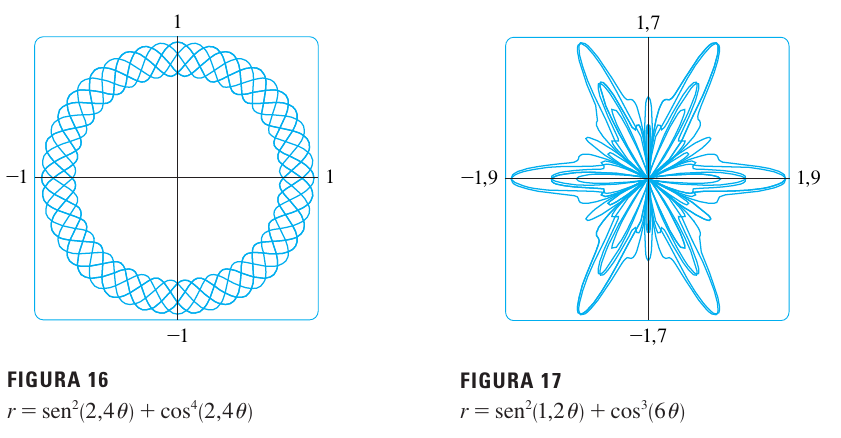
\includegraphics[scale=0.6]{figuras/introducao/curvas-polares1.png}
		\caption{}
	\end{figure}
	\item \textbf{{\color{blue}Aplicação na engenharia de som}}

Engenheiros de som usam coordenadas polares para descrever padrões de sons de microfones. Um padrão de captação em forma de {\color{blue}\textbf{cardioide}} captura principalmente a fonte sonora para a qual é apontado, como um cantor ou um instrumento, ao mesmo tempo que reduz a captação de ruído ambiente e sistemas de monitoramento de palco.

\begin{center}
	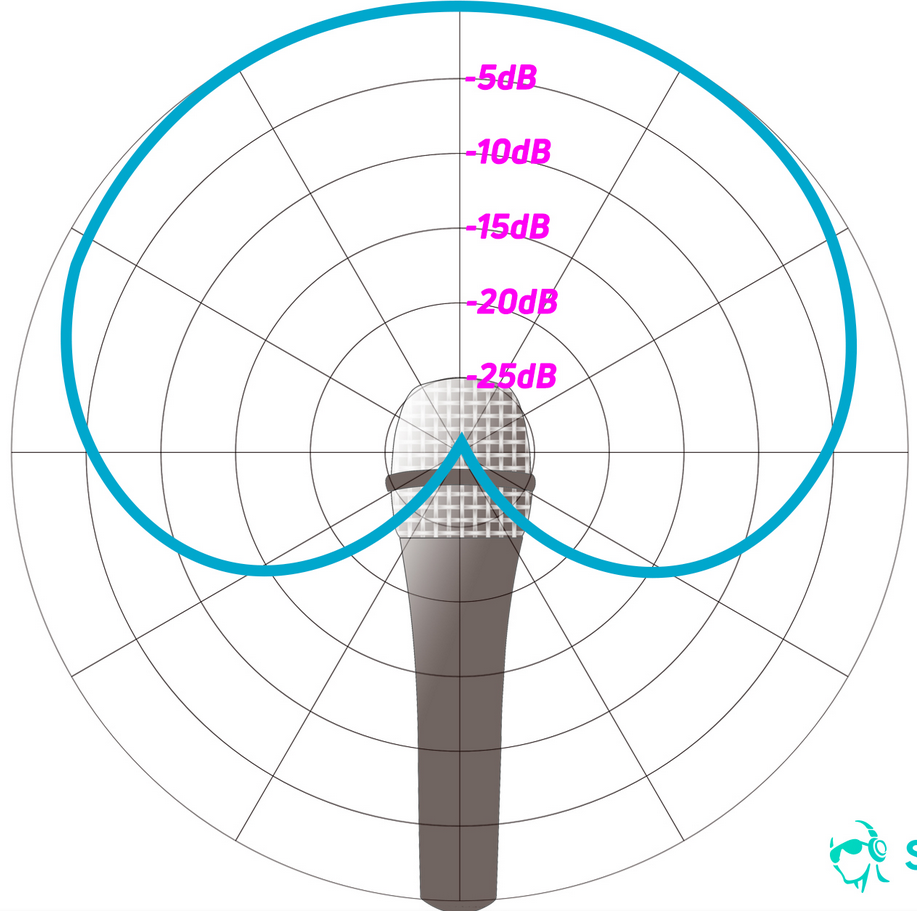
\includegraphics[scale=0.5]{figuras/introducao/cardioide-micro.png}
\end{center}
\end{itemize} 
	

\noindent\textbf{{\large Funções Vetoriais}}

\begin{itemize}
	\item \textbf{{\color{blue}Aplicação em Biologia}}
	
		Em 1953, James Watson e Francis Crick mostraram que a estrutura da molécula de
	{\color{blue}\textbf{DNA}} é de duas hélices circulares paralelas interligadas.

\begin{center}
	
\includegraphics[scale=0.7]{figuras/introducao/dna.png}
\end{center}



Sabendo-se o raio da hélice de DNA, o número de voltas e a altura de cada volta, usando o conceito de \dt{comprimento de curvas espaciais}, podemos calcular o comprimento da molécula de DNA.

\item \textbf{{\color{blue}Movimentos sobre curvas}}
	
No ensino médio, aprendemos que uma partícula em um  \dt{Movimento Circular Uniforme} tem velocidade constante {\color{teal} \(v\)}, mas para manter sua trajetória em um círculo de raio {\color{teal}\(R\)}, precisa de uma \dt{força centrípeta}, que gera a chamada \dt{aceleração centrípeta}, cuja fórmula é:
	\[
	{\color{teal} a_c=\frac{v^2}{R}}
	\]
	
	Contudo, para movimentos em um curva qualquer, essa aceleração tem uma \dt{forma vetorial}

	\[
	{\color{Goldenrod}\vec{a}}=v'\vec{T}+{\color{teal}\kappa v^2}\vec{N}
	\]

\begin{center}
	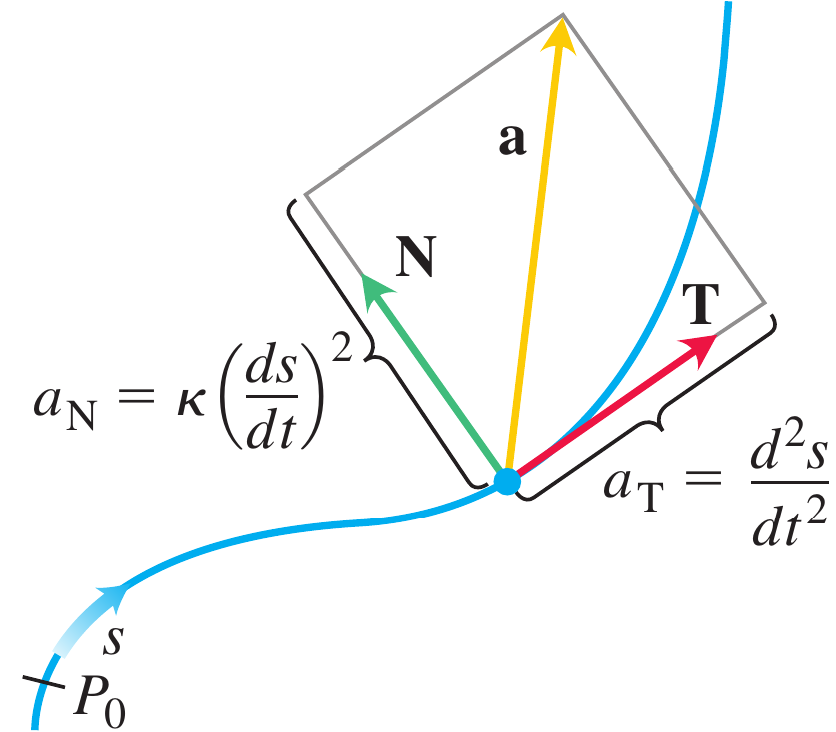
\includegraphics[scale=1.5]{figuras/introducao/curvatura.png}
\end{center}
\end{itemize}
\newpage

\noindent\textbf{{\large Funções de Várias Variáveis}}

\begin{itemize}
	\item \textbf{{\color{blue}Topografia}}
	
	As {\color{blue}curvas de nível} de funções de várias variáveis tem como exemplos de aplicações o estudo topográfico ou  das isotermas de regiões.
\begin{center}
	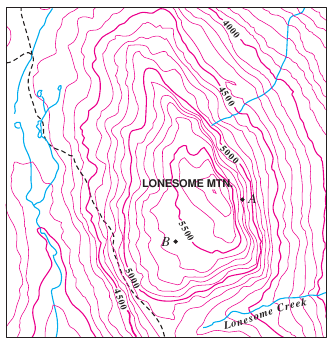
\includegraphics[scale=1]{figuras/nivel2.png}
\end{center}


\begin{center}
	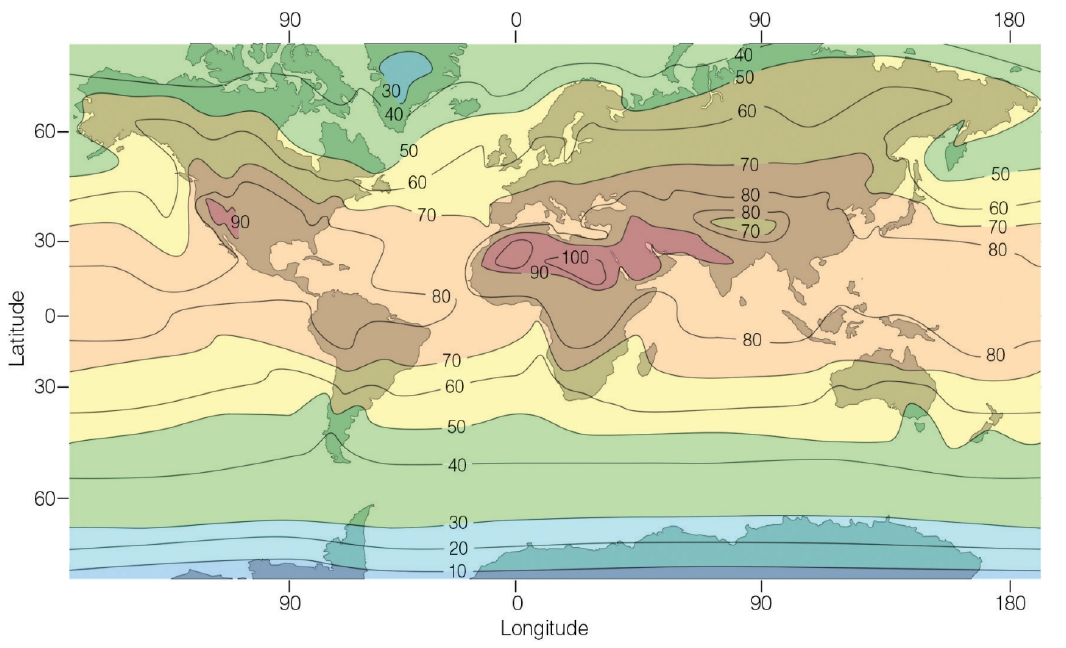
\includegraphics[scale=0.6]{figuras/nivel3.png}
\end{center}

\item \textbf{{\color{blue}Problema de Otimização: Produção restrita a um orçamento}}


A produção total \(P\) de certo produto depende do {\color{blue}custo \(x\) de trabalho empregado}  e da {\color{red}quantidade \(y\) de capital investido}. Na década de 1920 Charles
Cobb e Paul Douglas obtiveram o seguinte modelo
\[
P=b{\color{blue}x}^\alpha {\color{red}y}^{1-\alpha},
\]
onde \(b\) e \(\alpha\) são constantes positivas e \(\alpha<1\).

Para uma firma com função de produção e restrição orçamentária dadas por
\[
\begin{cases}
	P={\color{blue}x}^{2/3} {\color{red}y}^{1/3}\\
	{\color{blue}x}+ {\color{red}y}=3.78.
\end{cases}
\]
Teremos produção máxima \(P=2\) quando \({\color{blue}x=2.52}\) e \( {\color{red}y=1.26}\)
\begin{center}
	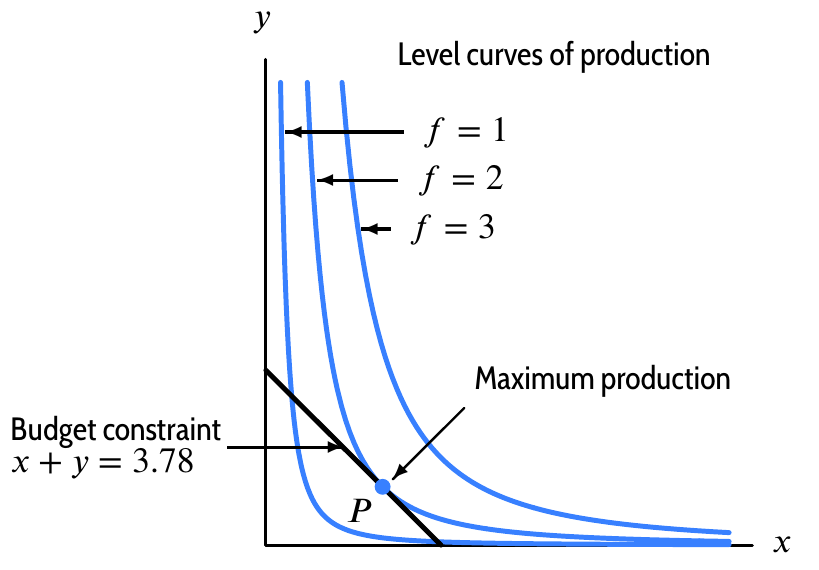
\includegraphics[scale=.7]{figuras/introducao/cobb-res.png}
\end{center}

\end{itemize}




%------------------------------------
\chapter{Elementos de Geometria Analítica}
\chapter{Superfícies}

\section{Revisão de Retas e Planos}

\textbf{{\large Equação Paramétrica de uma Reta}}


Sabemos que uma reta $r$ pode ser inteiramente descrita por uma {\color{blue} equação vetorial paramétrica}
\[P={\color{red}A}+t{\color{blue}\vec{v}},\ t\in \R.\]
\begin{center}
	\begin{tikzpicture}
		\tikzset{>=latex}
		\draw[thick] (-1,-1) -- (2,2);
		\node[left] at (2,2) {r};
		\draw[fill=red] (0,0) circle [radius=1.5pt];
		\node[above left] at (0,0) {$\textcolor{red}{A}$};
		\draw[thick, blue,->] (2,0) -- (0.7+2,0.7);
		\node[blue, right] at (0.7+2,0.7) {$\vec{v}$};
		\draw[fill=black] (1.5,1.5) circle [radius=1.5pt];
		\node[above left] at (1.5,1.5) {$P$};
		\draw[thick, blue,->] (0,0) -- (1.5,1.5);	
		
	\end{tikzpicture}
\end{center}
onde ${\color{red} A}$ é um ponto fixado de $r$ e  ${\color{blue}\vec{v}}$ é um vetor diretor desta reta.\\


\noindent\textbf{Em coordenadas:}

Se	$P=(x,y)$, $\textcolor{red}{A=(x_0,y_0)}$ e $\textcolor{blue}{\vec{v}=(a,b)}$
\[	r: \left\{\begin{array}{l}
	x=\textcolor{red}{x_0}+\textcolor{blue}{a}t\\
	y=\textcolor{red}{y_0}+\textcolor{blue}{b}t,\  t\in \R.
\end{array}\right.\]

Se 	$P=(x,y,z)$, $\textcolor{red}{A=(x_0,y_0,z_0)}$ e $\textcolor{blue}{\vt{v}=(a,b,c)}$
\[r:	\left\{\begin{array}{l}
	x=\textcolor{red}{x_0}+\textcolor{blue}{a}t\\
	y=\textcolor{red}{y_0}+\textcolor{blue}{b}t\\
	z=\textcolor{red}{z_0}+\textcolor{blue}{c}t,\  t\in \R.
\end{array}\right.\]
Estas equações são chamadas simplesmente \dt{equações paramétricas  da reta} $r$.


\begin{exeb}{}{exer4}
	\begin{enumerate}
		\item Determinar  as equações paramétricas da reta $r$ que passa pelos
		pontos $A = (1, 2, -2)$ e $B = (-1, 4, 2)$.
		
		\item Sejam $A=(0,1,8), B=(-3,0,9)$ e $r: X=(1,2,0)+t(1,1,-3)$. Determine o ponto $C$ de $r$ tal que $A,B$ e $C$ sejam vértices de um triângulo retângulo com ângulo reto no vértice $A$.
	\end{enumerate}
\end{exeb}
\newpage

\noindent\textbf{{\large Equação Cartesiana do Plano no Espaço}}

Sejam  ${\color{red}A=(x_0,y_0,z_0)}$  um ponto de um plano em $\R^3$, $\textcolor{blue}{\vt{n}=(a,b,c)}\perp \pi$, então os pontos e  $P=(x,y,z)$do plano devem satisfazer a seguinte \dt{equação cartesiana}
\[{\color{blue}a}x+{\color{blue}b}y+{\color{blue}c}z+{\color{red}d}=0\]
\begin{center}
	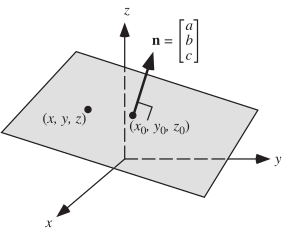
\includegraphics[scale=0.9]{figuras/normal-vector.png}
\end{center}

\begin{exeb}{}{} Vamos recordar a resolução dos seguintes problemas:
	
	\begin{enumerate}
		\item Determine a equação do plano que passa por $A=(1,3,2)$, $B=(3,-1,6)$ e $C=(5,2,0)$. 
		
		\item Determine o ponto da reta 
		\[r: \begin{cases} x=2+3t,\\ y=-4,\\ z=5+t, \ \ t\in \R. \end{cases}
		\]
		que intercepta o plano $4x+5y-2z=18$.
		
		
		\item Determine a equação do plano que passa pelo ponto $A=(1,0,1)$ e é perpendicular à reta $r: X=(-1,1,2)+t(-1,2,1),\ t\in \R$.
		
	\end{enumerate}
\end{exeb}
\newpage

\begin{exerb}{}{} Resolve os exercícios:
	\begin{enumerate}
		\item Determine uma equação para o plano que passa pelos pontos $A=(0,1,1)$, $B=(1,0,1)$ e $C=(1,1,0)$.
		
		\item Determine as equações paramétricas da reta dada pela interseção dos planos
		$x+y+z=1$ e $x-2y+3z=1$.
		
		\item Determine as equações paramétricas da reta que passa pelo ponto $(1,0,6)$ e é perpendicular ao plano $x+3y+z=5$.
	\end{enumerate}
\end{exerb}
\newpage

\section{Superfícies}



\noindent\textbf{{\large Superfícies Cilíndricas}}

Uma \dt{superfície cilíndrica} é aquela gerada por uma reta $\ell$ que se move ao longo de uma curva plana dada, de modo que a reta $\ell$ sempre esteja paralela a uma reta fixa. A reta $\ell$ é chada de \dt{geratriz} e a curva de \dt{diretriz}.

\begin{exeb}{}{}
	A equação $z=x^2$ em $\R^3$ representa a seguinte superfície cilíndrica.
	
	\begin{center}
		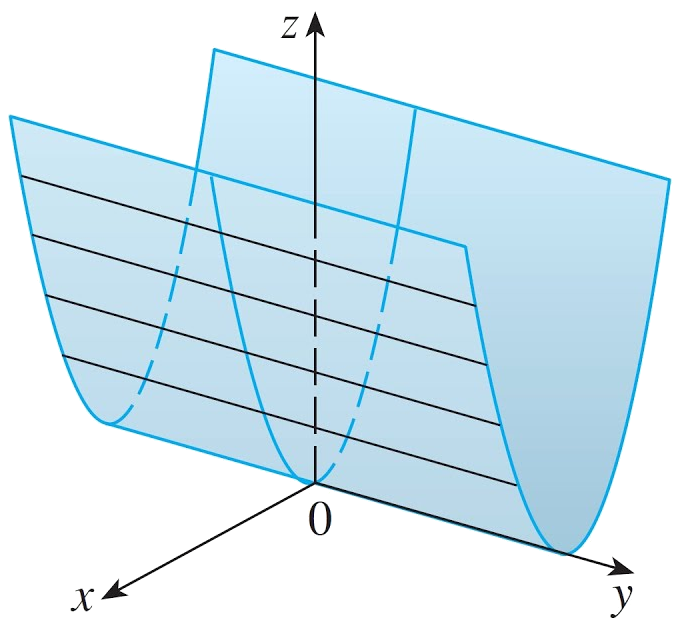
\includegraphics[scale=1]{figuras/cilindro-ex1.png}
	\end{center}
\end{exeb}

\begin{exeb}{}{}
Esboce as superfícies
	\begin{enumerate}[(a)]
		\item $y^2+z^2=1$
		\item $z=1-y^2$
	\end{enumerate}
\end{exeb}
\newpage

\noindent\textbf{{\large Superfícies Quádricas}}

Uma \dt{superfície quádrica} é o gráfico de uma equação do segundo grau a três variáveis, isto é, uma equação da forma:
\begin{equation*}
	{\color{red}A}x^2+{\color{red}B}y^2+{\color{red}C}x^2+{\color{red}D}xy
	+{\color{red}E}xz+{\color{red}F}yz+{\color{red}G}x+{\color{red}H}y+
	{\color{red}I}z+{\color{red}J}=0,
\end{equation*}
onde pelo menos um dos coeficientes ${\color{red}A}, {\color{red}B}, 
{\color{red}C}, {\color{red}D}, {\color{red}E}$ ou ${\color{red}F}$ é {\color{blue} não nulo}.

\begin{minipage}{0.5\textwidth}
	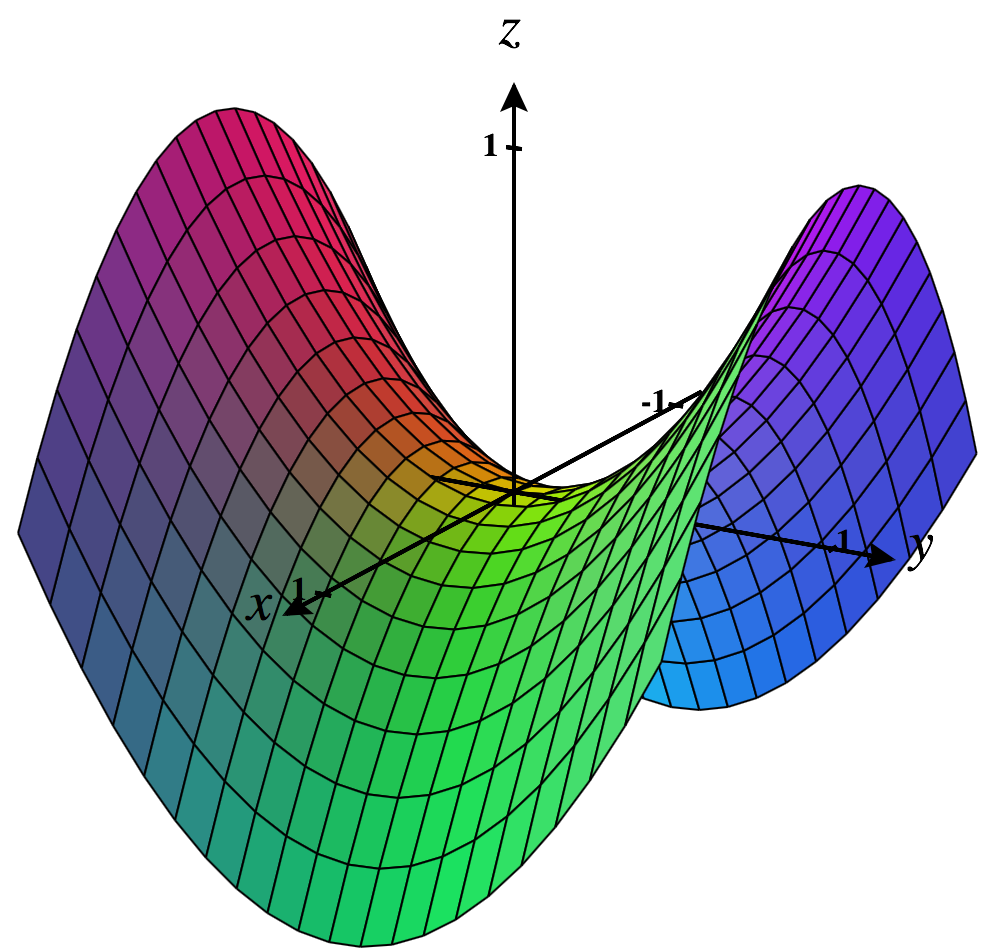
\includegraphics[scale=0.13]{figuras/quadricas/parab-hip.png}
\end{minipage}
\begin{minipage}{0.4\textwidth}
	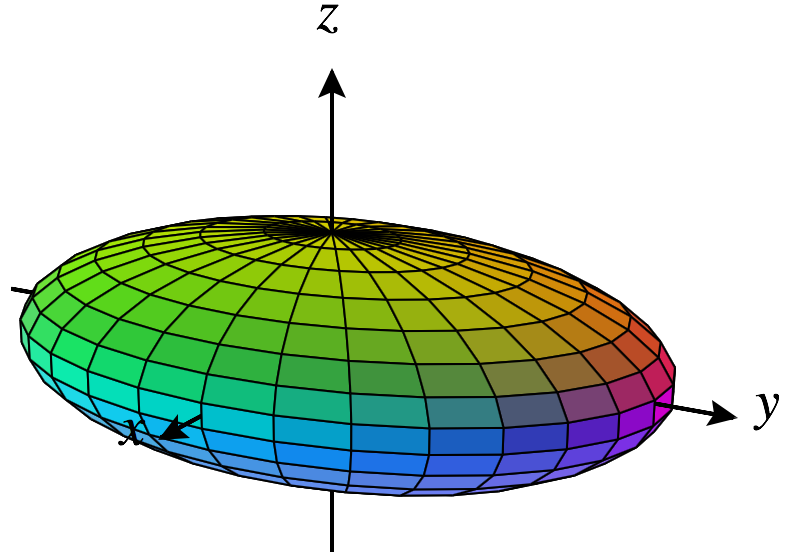
\includegraphics[scale=0.8]{figuras/quadricas/elipsoide.png}
\end{minipage}
\bigskip

\noindent\textbf{Forma Padrão}

Através de uma rotação e uma translação é possível colocar a {\color{blue}superfície quádrica} em uma das chamadas {\color{blue} formas padrão}.

\begin{center}
	\textbf{Elipsoide:} \(\frac{x^2}{a^2}+\frac{y^2}{b^2}+\frac{z^2}{c^2}=1\)
	\bigskip
	
	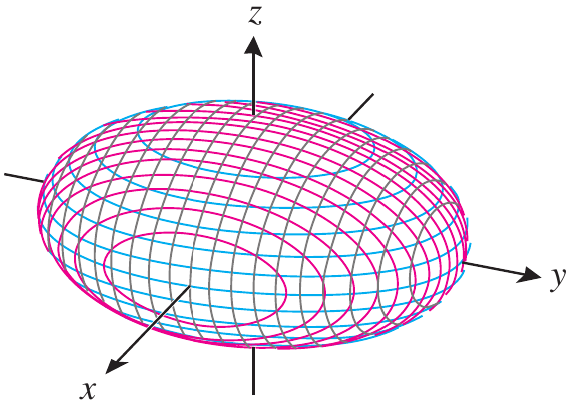
\includegraphics[scale=0.5]{figuras/quadricas/elipsoide-padrao.png}
\end{center}

\hrulefill


\begin{center}
	\textbf{Hiperboloide de uma folha:} \(\frac{x^2}{a^2}+\frac{y^2}{b^2}-\frac{z^2}{c^2}=1\)
	\bigskip
	
	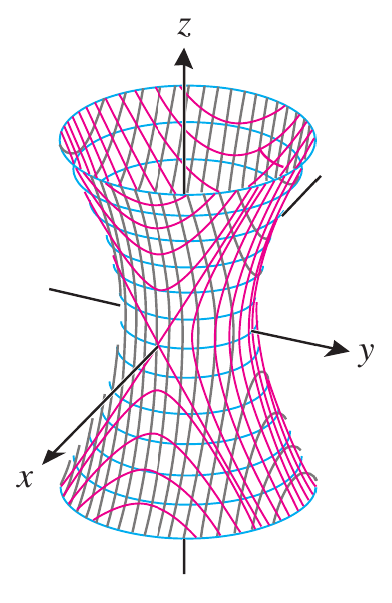
\includegraphics[scale=0.5]{figuras/quadricas/hiperboloide1-padrao.png}
\end{center}

\hrulefill

\begin{center}
	\textbf{Hiperboloide de duas folha:} \(-\frac{x^2}{a^2}-\frac{y^2}{b^2}+\frac{z^2}{c^2}=1\)
	\bigskip
	
	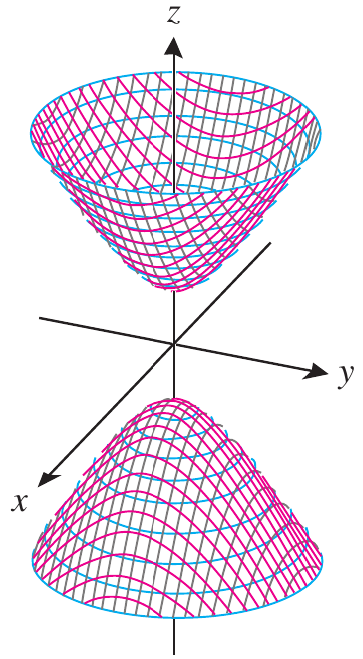
\includegraphics[scale=0.5]{figuras/quadricas/hiperboloide2-padrao.png}
\end{center}

\hrulefill

\begin{center}
	\textbf{Cone:} \(z^2=\frac{x^2}{a^2}+\frac{y^2}{b^2}\)
	\bigskip
	
	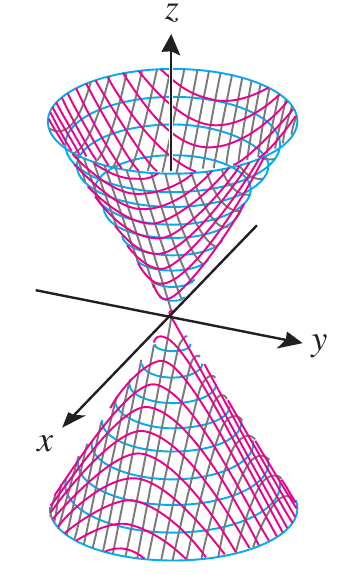
\includegraphics[scale=0.5]{figuras/quadricas/cone-padrao.png}
\end{center}

\hrulefill

\begin{center}
	\textbf{Paraboloide Elíptico:} \(z=\frac{x^2}{a^2}+\frac{y^2}{b^2}\)
	\bigskip
	
	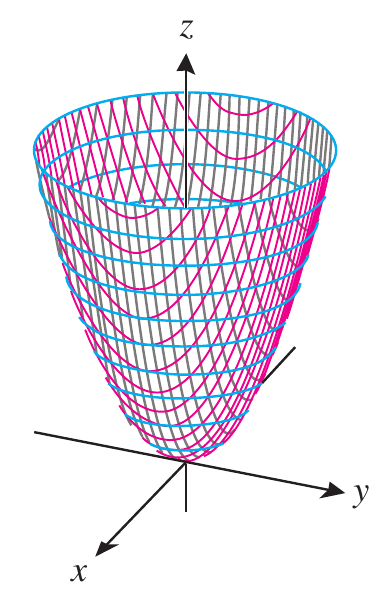
\includegraphics[scale=0.5]{figuras/quadricas/paraboloide-padrao.png}
\end{center}

\hrulefill

\begin{center}
	\textbf{Paraboloide Hiperbólico:} \(z=\frac{x^2}{a^2}-\frac{y^2}{b^2}\)
	\bigskip
	
	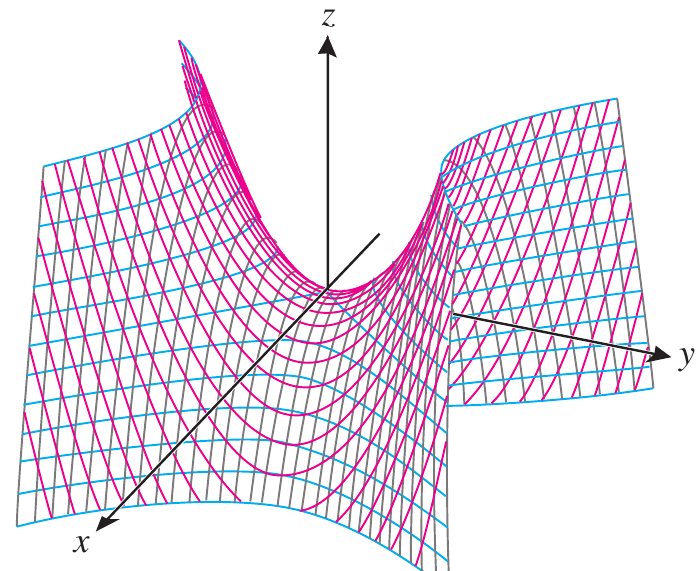
\includegraphics[scale=0.5]{figuras/quadricas/paraboloide-hiperbolico-padrao.png}
\end{center}

\begin{center}

\textbf{Resumo}

\begin{tabular}{|c|c|c|}
	\hline
	Equação & Característca  & Classifciação    \\
	\hline
	\(\frac{x^2}{a^2}+\frac{y^2}{b^2}+\frac{z^2}{c^2}=1\) & \makecell{3 termos quadráticos \(=1\) \\ Sem sinal negativo } & Elipsoide \linebreak    \\
	\hline
	\(\frac{x^2}{a^2}+\frac{y^2}{b^2}{\color{red}-}\frac{z^2}{c^2}=1\)& \makecell{3 termos quadráticos \(=1\) \\ {\color{red}1 sinal negativo} }  & \makecell{Hiperboloide \\ de {\color{red}  1 folha} }    \\
	\hline
	\({\color{red}-}\frac{x^2}{a^2}+\frac{y^2}{b^2}{\color{red}-}\frac{z^2}{c^2}=1\) & \makecell{3 termos quadráticos \(=1\) \\ {\color{red} 2 sinais negativo} }  & \makecell{Hiperboloide \\ de {\color{red} 2 folha} }    \\
	\hline
	\( \frac{x^2}{a^2}+\frac{y^2}{b^2}=\frac{z^2}{c^2} \)& \makecell{2 termos quadráticos  \\ \(=\) ao terceiro }
	& Cone   \\
	\hline
	\( {\color{blue} z}=\frac{x^2}{a^2}+\frac{y^2}{b^2} \)& \makecell{{\color{blue} 1 termo linear} \(=\) 2 
		quadráticos 
		\\ com mesmo sinal }   & \makecell{{\color{blue} Paraboloide}\\ Elíptico}   \\
	\hline
	\(  {\color{blue} z}=\frac{x^2}{a^2}-\frac{y^2}{b^2} \)& \makecell{{\color{blue} 1 termo linear} \(=\) 2 
		quadráticos 
		\\ com {\color{red} sinais opostos} }   & \makecell{ {\color{blue} Paraboloide}\\  {\color{red} Hiperbólico}}   \\
	\hline
\end{tabular}
\end{center}


\begin{exeb}{}{}
	Reconheça e esboce às quádricas
	\begin{enumerate}
		\item \(z=4x^2+y^2\)
		\item \(z=y^2-x^2\)
		\item \(\displaystyle\frac{x^2}{4}+y^2-\frac{z^2}{4}=1\)
	\end{enumerate}
\end{exeb}


\section{Coordenadas Polares}

Um sistema de \dt{coordenadas polares} é estabelecido da seguinte forma:

\begin{enumerate}
	\item Fixamos um ponto no plano, conhecido como \dt{polo} (ou origem), denotado por $O$.
	
	\item Fixamos uma semi-reta a partir de $O$, chamada \dt{eixo polar}.
\end{enumerate}

As \dt{coordenadas polares} de ponto {\color{red}$P$} do plano são formadas por um par ordenado $(r,\theta)$, sendo $r$ a distância de {\color{red}$P$} a $O$ e $\theta$ o ângulo entre o eixo polar e a reta $OP$.
\medskip


\begin{center}
	\begin{tikzpicture}[scale=3]
	\tikzset{>=latex}
	
	\coordinate (A) at ({2*cos(45)},{2*sin(45)});
	\coordinate (O) at (0,0);
	\coordinate (i) at (2,0);
	
	\pic[draw,angle eccentricity=1.5,->] {angle = i--O--A};
	
	\draw[->] (0,0) -- (3,0) node[right] {eixo polar};
	
	\node[thick] at (0.8,0.3) {$\theta$};
	\draw[very thick,blue] (0,0) -- ({2*cos(45)},{2*sin(45)});
	
	\node at (0.5,1) {$r$};
	\node[right] at (A) {$(r,\theta)$};
	\fill[red] (A) circle (1pt);
	
	\node[left] at (0,0) {$O$};
	
\end{tikzpicture}
\end{center}

{\large\textbf{Convenções}}
\begin{itemize}
	\item Um ângulo é \dt{positivo} se for medido no sentido anti-horário a partir do eixo polar e {\color{red}negativo} se for medido no sentido horário.
	
	\item $(0,\theta)$ representa o {\color{blue}polo} para qualquer valor de $\theta$.
	
	\item Se $r<0$, a coordenada $(r,\theta)$ corresponde ao simétrico, em relação à origem, do ponto $(|r|,\theta)$.
	
	
	\centering
	
	\begin{tikzpicture}
		\tikzset{>=latex}
		
		\coordinate (A) at ({2*cos(45)},{2*sin(45)});
		\coordinate (O) at (0,0);
		\coordinate (i) at (2,0);
		\coordinate (B) at ({2*cos(45+180)},{2*sin(45+180)});
		
		\pic[draw,->,angle radius=1cm] {angle = i--O--A};
		
		\pic[draw,->] {angle = i--O--B};
		
		\draw[->] (0,0) -- (3,0) node[right] {eixo polar};
		
		\node[thick] at (1.2,0.3) {$\theta$};
		\draw[very thick,dashed] (0,0) -- ({2*cos(45)},{2*sin(45)});
		
		\node at (0.5,1) {$|r|$};
		\node[right] at (A) {$(|r|,\theta)$};
		\fill[black] (A) circle (2pt);
		
		\node[below] at (0,0) {$O$};
		
		\draw[very thick,blue] (0,0) -- ({2*cos(45+180)},{2*sin(45+180)});
		
		\node[left] at (B) {$(r,\theta)$};
		\fill[red] (B) circle (2pt);
		\node at ({0.8*cos(90+45)},{0.8*sin(90+45)}) {$\theta +\pi$};
		
	\end{tikzpicture}
\end{itemize}
%-------------------------------------
\chapter{Funções Vetoriais}
\section{Funções Vetoriais e Limites}

\begin{definb}{}{}
Uma \dt{função vetorial} é uma função cujo domínio é um conjunto de números reais e cuja imagem é um conjunto de vetores em $\R^n$, denotada por:
\[\begin{array}{lcl}
\vec{r}: & D\subset \R &  \longrightarrow \R^n\\
         & t           & \longmapsto \vec{r}(t)=(f_1(t),f_2(t),\ldots,f_n(t)).
\end{array}\]

As funções $f_1,\ldots,f_n$ são chamada \dt{funções componentes}.
\end{definb}

\begin{exeb}{}{}
\begin{enumerate}
\item $\vec{r}(t)=(t,t)$, $t\in \R$.
\item $\vec{r}(t)=(t,1,0)$, $t\geq 0$.
\end{enumerate}
\end{exeb}
\newpage


\marcador{subsection}{Limite e Continuidade}

\begin{definb}{}{}
Sejam $\vec{r}(t)=(f_1(t),f_2(t),\ldots,f_n(t))$ uma função vetorial com domínio $D$. Definimos o \dt{limite de $\vec{r}(t)$ quanto $t$ tende a $a\in D$} por
\[\lim\limits_{t\to a}\vec{r}(t)=\left(\lim\limits_{t\to a}f_1(t),\ldots,\lim\limits_{t\to a}f_n(t)\right), \]
desde que o limite das funções componentes existam.
\end{definb}

\begin{exerb}{}{}
Determine $\lim\limits_{t\to 0}\vec{r}(t)$, onde $\vec{r}(t)=(1+t^3, te^{-t})$.
\end{exerb}
\vspace{5cm}


\begin{definb}{}{}
Uma função vetorial $\vec{r}$ é \dt{contínua em $a$} se $\lim\limits_{t\to a}\vec{r}(t)=\vec{r}(a)$.
\end{definb}
Em vista desta definição, uma função $\vec{r}$ é {\color{blue}contínua em $a$} se, e somente se, cada uma de suas {\color{blue}componentes é contínua em $a$}.


\newpage



\marcador{subsection}{Curvas Parametrizadas}

Quando uma função vetorial \dt{$\vec{r}(t)=(f(t),g(t))$}, está definida em um intervalo $I$ da reta e  é \dt{contínua}, então o conjunto {\color{red}$C$} de todos os pontos $(x,y)$ do plano tais que
\begin{equation}\label{parametricas}
x={\color{blue}f(t)}\ \text{ e } y={\color{blue}g(t)}
\end{equation}
quando $t$ varia formam uma {\color{red}curva no plano}. As equações em  {\color{red} \eqref{parametricas}} são ditas {\color{red} equações paramétricas de $C$}, \dt{\(\vec{r}\)} é dita ser uma {\color{red}parametrização de $C$} e $t$ é chamado de  {\color{red} Parâmetro}.
\begin{exeb}{}{}
Determine as curvas parametrizadas por:
\begin{enumerate}
\item $\vec{r}(t)=(\cos(t),\sin(t))$, $t\in [0,2\pi]$.
\item $\vec{r}(t)=(\cos(2t),\sin(2t))$, $t\in [0,2\pi]$.

\end{enumerate}
\end{exeb}
\blfootnote{
Veja como plotar curvas parametrizadas usando Python \href{https://reginaldodr.github.io/academic/posts/curvas-parametricas/curvas-parametricas.html}{Curvas parametrizadas com Python}
}

\newpage


\begin{caixaazul}{Parametrização do Gráfico de uma Função}
O gráfico de qualquer função ${\color{blue}y=f(x)}, x\in I\subset\R$, pode ser parametrizado de forma natural usando a variável {\color{red}$x$ como parâmetro}, da seguinte forma:
\[\vec{r}({\color{red}t})=({\color{red}t},{\color{blue}f(t)}),\ {\color{red}t\in I}.\]
\end{caixaazul}

\begin{exeb}{}{}
 Determine uma parametrização para as curvas:
\begin{enumerate}[(a)]
\item A parábola $y=x^2$.
\item O gráfico da função \(y=\cos(x)\).
\item \(e^y-x^2=1\).
\item \(x=y^2+y\)
\end{enumerate}
\end{exeb}
\newpage




Se em uma equação polar {\color{blue}a coordenada $r$ estiver em função de $\theta$}, isto é, {\color{blue}$r=f(\theta)$}, então podemos usar {\color{red}$\theta$ como parâmetro} e parametrizar a curva representada pela equação polar da seguinte forma:

\begin{center}
\destaque{
\(
\vec{\alpha}({\color{red}\theta})=f({\color{red}\theta})(\cos {\color{red}\theta},\sin {\color{red}\theta})
\)
}
\end{center}

\begin{exeb}{}{}
Determine uma parametrização para a  cardioide $r=1+\cos \theta$
%\[\vec{\alpha}(\theta)=(r\cos \theta,r\sin \theta)=(1+\cos (\theta))(\cos \theta,\sin \theta),\ \theta\in [0,2\pi].\]

\end{exeb}



\vfill
\begin{casab}{}{}
\begin{enumerate}
\item  Determine uma parametrização para o segmento de reta que entre os pontos $(1,0)$ e $(2,5)$.
\item Determine a curva parametrizada por $\vec{r}(t)=(2\cos(t),\sin(t))$, $t\in [0,2\pi]$.
\item		Esboce a curva que é representada pelas equações polares abaixo.
\begin{enumerate}
\item $r=2\cos\theta$

\item $r=\cos 2\theta$ (rosácea de quatro pétalas)
\end{enumerate}
\end{enumerate}
\end{casab}
\newpage


\marcador{subsection}{Curvas Parametrizadas no Espaço}

Quando uma função vetorial {\color{blue}$\vec{r}(t)=(f(t),g(t),h(t))$}, está definida em um intervalo $I$ da reta e  é \dt{contínua}, então o conjunto {\color{red}$C$} de todos os pontos $(x,y,z)$ do plano tais que
\begin{equation}\label{parametricas2}
x={\color{blue}f(t)},\  y={\color{blue}g(t)}\ \text{ e } z={\color{blue}h(t)}
\end{equation}
quando $t$ varia formam uma {\color{red}curva no espaço}. As equações em  {\color{red} \eqref{parametricas2}} são ditas {\color{red} equações paramétricas de $C$}, ${\color{blue}\vec{r}}$ é dita ser uma {\color{red}parametrização de $C$} e $t$ é chamado de  {\color{red} Parâmetro}.

\begin{center}
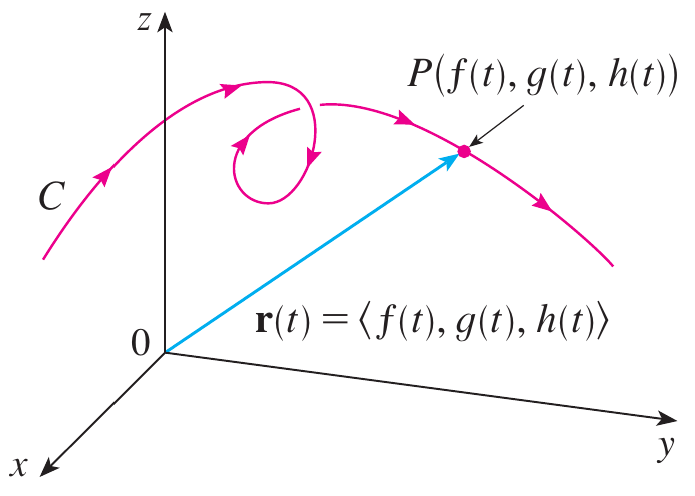
\includegraphics[scale=.5]{figuras/curvas/param-curvas-espaco.png}
\end{center}


\begin{exeb}{}{}
Determine as curvas parametrizadas por:
\begin{enumerate}
\item $\vec{r}(t)=(1,t,2t)$, $t\in (0,1)$.
\item $\vec{r}(t)=(\cos(t),\sin(t),t)$, $t\in [0,2\pi]$.
\end{enumerate}
\end{exeb}
\newpage


\begin{caixaazul}{Hélices}
A curva do exemplo anterior é uma \dt{hélice}. Existem vários tipos de hélices, as mais simples são as \dt{hélices circulares com passo constante}, cuja  parametrização e dada por
\[\vec{r}(t)=({\color{red}a}\cos(t),{\color{red}a}\sin(t),{\color{blue}b}t),\]
onde ${\color{red}a},{\color{blue}b}$ são constantes.

As hélices aparecem em diversas aplicações, como por exemplo no formato de molas e no modelo de DNA que é formado por uma dupla hélice.
\end{caixaazul}
\bigskip

\begin{minipage}{0.33\textwidth}
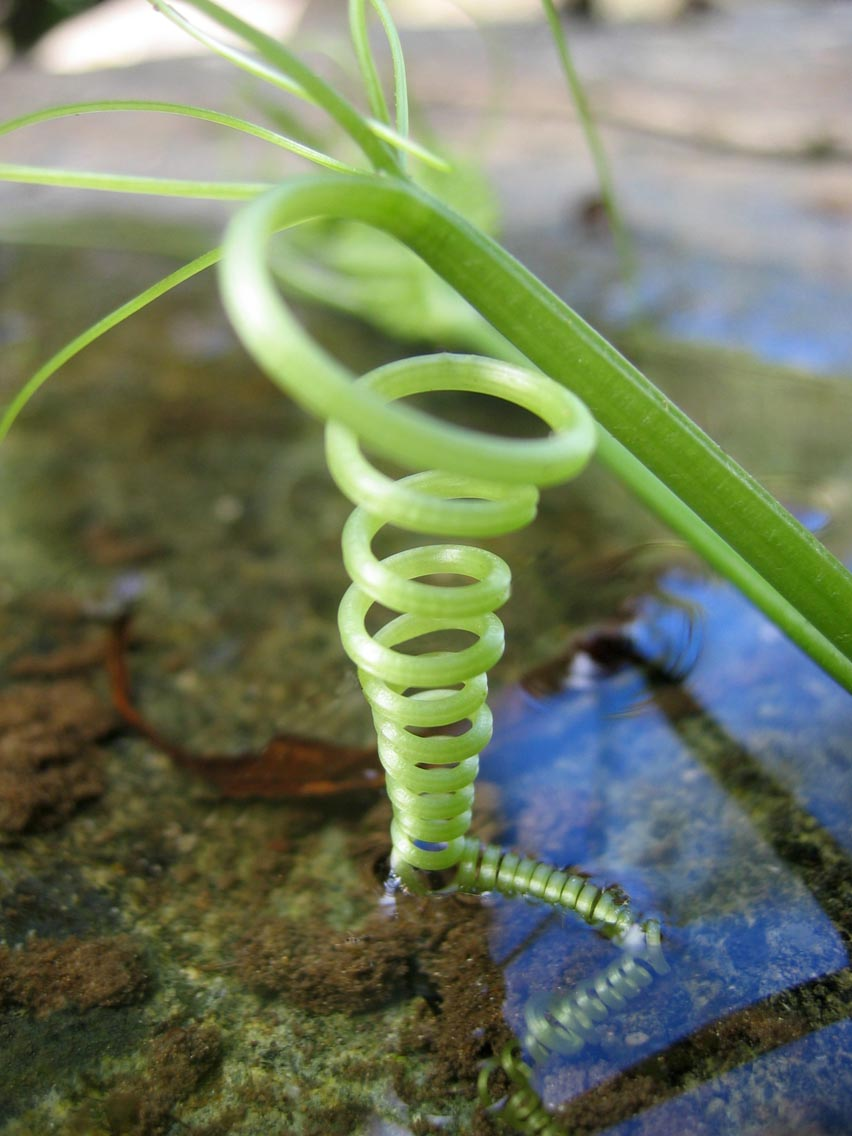
\includegraphics[scale=0.2]{figuras/DirkvdM_natural_spiral.jpg}
\end{minipage}
\begin{minipage}{0.35\textwidth}
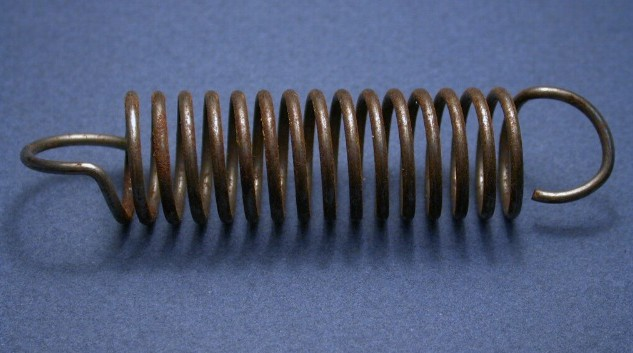
\includegraphics[scale=1]{figuras/mola.jpg}
\end{minipage}
\begin{minipage}{0.33\textwidth}

\includegraphics[scale=1]{figuras/introducao/dna.png}
\end{minipage}

\newpage

\marcador{subsection}{Parametrização por inteseção de superfícies}


\begin{itemize}
\item {\color{red}NÃO} existe equação cartesiana de curvas em {\color{red}\(\R^3\)};

\item Uma equação cartesiana no {\color{red}\(\R^3\)} {\color{red}SEMPRE} representa uma superfície.

\begin{center}
{\color{blue}\(y+z=2\) é um plano} e
{\color{orange}\(x^2+y^2=1\) é um cilindro.}
\end{center}
\end{itemize}

Muitas curvas no espaço, podem ser parametrizadas via interseção de duas superfícies.

\begin{center}
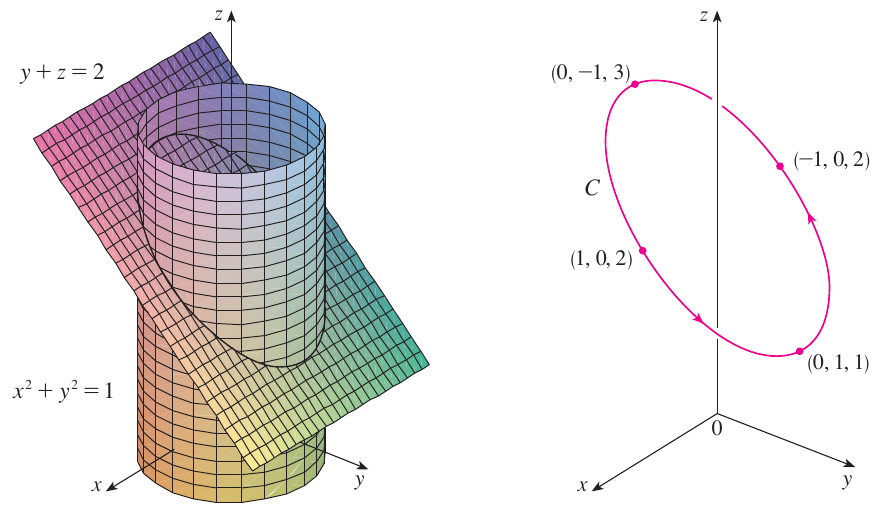
\includegraphics[scale=0.7]{figuras/curvas/cilindro-plano.png}
\end{center}

\begin{exeb}{}{}
 Determine uma equação vetorial que represente a curva obtida pela interseção das superfícies:
\begin{enumerate}
\item Os planos: \(y+z=1\) e \(x+y=1\);

\item O cone \(z=\sqrt{x^2+y^2}\) e o plano \(x+y=1\);

\item  da esfera $x^2+y^2+z^2-2z=3$ com o plano $z=\frac{3}{2}$;

\item do cilindro $x^2+y^2=1$ com o plano $y+z=2$;

\item do paraboloide $x^2+y+z^2=1$ com o cilindro $y=x^2$.

%\item  da esfera $x^2+y^2+z^2=1$ com o cilindro $y=x^2$.
\end{enumerate}
\end{exeb}

%---------------------------------------
\chapter{Funções de Várias Variáveis}

%\appendix
%\include{apendiceA}

%\backmatter
%\bibliographystyle{alpha}
%\bibliography{bibliografia}
%\addcontentsline{toc}{chapter}{Bibliografia}

\printindex
\end{document}

%%%%%%%%%%%%%%%%%%%%%%%%%%%%%%%%%%%%%%%%%%%%%%%%%
